%%%%%%%%%%%%%%%%%%%%%%%%%%%%%%%%%%%%%%%%%%%%%%%%%%%%%%%%%%%%%%%%%%%%%%
% Lớp 11 | Đạo hàm | Các quy tắc đạo hàm
% Dạng 1D7?2-5: Tiếp tuyến chưa biết tiếp điểm và hệ  số góc
% Số câu: 32  (sinh tự động bởi tach_cau.py; từ nay thầy sửa trực tiếp file này)
%%%%%%%%%%%%%%%%%%%%%%%%%%%%%%%%%%%%%%%%%%%%%%%%%%%%%%%%%%%%%%%%%%%%%%

%%%%%%%%%%%%%%%% TRẮC NGHIỆM 4 PHƯƠNG ÁN %%%%%%%%%%%%%%%%

% nguồn: Ok_Toan11_TracNghiem_Lan2
\begin{ex}%[1D7H2-5]%[ma:7c8ba512]
	Phương trình tiếp tuyến của đồ thị hàm  số $y=\dfrac{x+1}{x-2}$ tại điểm có tung độ bằng $-2$ là
	 \choice
		 {$y=3x+1$}
		 {$y=-3x-1$}
		{\True  $y=-3x+1$}
		{$y=-3x+3$} 
	\loigiai{ 
		Gọi $M(x_0;y_0)$ thuộc đồ thị của hàm số $y=\dfrac{x+1}{x-2}$. Khi  đó,
		\begin{align*}
			y_0=-2\Leftrightarrow  \dfrac{x_0+1}{x_0-2}=-2\Leftrightarrow x_0+1=-2(x_0-2)\Leftrightarrow x_0=1
		\end{align*}
		Suy ra $M(1;-2)$.\\ 
		Ta có  $y'=\dfrac{-3}{(x-2)^2}$, suy ra $y'(1)=-3$.\\
		 Do đó, phương trình tiếp tuyến của đồ thị hàm số $y=\dfrac{x+1}{x-2}$ tại $M(1;-2)$ là
		\begin{align*}
			 y=-3(x-1)-2=-3x+1.
		\end{align*}
	 }
\end{ex}

% nguồn: Ok_TracNghiemLop11_Lan1
\begin{ex}%[1D7H2-5]%[ma:f68a4a3d]
	Cho hàm số $y=-x^3+3x^2+2x-5$ có đồ thị  là $(C)$. Hệ số góc của tiếp tuyến của đồ thị $(C)$ tại điểm có hoành độ $x_0=-2$ bằng
	 \choice
		 {$1$}
		 {$2$}
		 {$22$}
		{\True  $-22$}
	\loigiai{ 
		Ta có $y'=-3x^2+6x+2$.\\ 
		Hệ số góc của tiếp tuyến của đồ thị $(C)$ tại điểm có hoành độ $x_0=-2$ là  $k=y'(-2)=-3(-2)^2+6(-2)+2=-22$.
	 }
\end{ex}

% nguồn: Ok_TracNghiemLop11_Lan1
\begin{ex}%[1D7H2-5]%[ma:82a9377c]
	 Tiếp tuyến của đồ thị hàm số $ y=x^3-3x+2$ vuông góc với đường thẳng $ y=-\dfrac{1}{9}x$ là
	\choice 
		{$y=-\dfrac{1}{9}x+18$;  $\,y=-\dfrac{1}{9}x+5$}
		{$y=-\dfrac{1}{9}x+18$; $y=\dfrac{1}{9}x-14$} 
		{\True $y=9x+18$; $y=9x-14$} 
		{$y=9x+18$; $y=9x+5$} 
	\loigiai{ 
		 Ta có $y'=3x^2-3$.\\
		Gọi $\Delta  $ là tiếp tuyến cần tìm và $M_0\left(x_0;{y_0}\right)$ là tiếp điểm. Do $\Delta\perp d\colon y=-\dfrac{1}{9}x$ nên
		$$k_\Delta\cdot\left(-\dfrac{1}{9}\right)=-1\Leftrightarrow{k_\Delta}=9\Leftrightarrow  3x_0^2-3=9\Leftrightarrow{x_0}=\pm 2.$$
		\begin{itemize}
			\item Với  $x_0=2\Rightarrow{y_0}=4\Rightarrow $ tiếp điểm $M_0\left(2;4\right)$, vậy phương trình tiếp tuyến là $$\Delta \colon y=9x-14.$$
			\item Với $x_0=-2\Rightarrow{y_0}=0\Rightarrow  $ tiếp điểm $M_0\left(-2;0\right)$, vậy phương trình tiếp tuyến là $$\Delta \colon y=9x+18.$$
		\end{itemize}
	 }
\end{ex}

% nguồn: Ok_Toan11_TracNghiem_Lan2
\begin{ex}%[1D7V2-5]%[ma:9eaa0e0d]
	Tính tổng $S$ tất cả giá trị của tham số $m$ để đồ  thị hàm số $f(x)=x^{3}-3mx^{2}+3mx+m^{2}-2m^{3}$ tiếp xúc với trục hoành.
	 \choice
		{$S=\dfrac{4}{3}$} 
		 {$S=1$}
		 {$S=0$}
		{\True  $S=\dfrac{2}{3}$}
	 \loigiai{
		\begin{itemize}
			\item Đồ thị hàm  số $f(x)$ tiếp xúc với trục hoành khi và chỉ khi hệ phương trình sau có nghiệm
			\begin{eqnarray*}
				\heva{& f(x)=0 \\ & f'(x)=0}\Leftrightarrow \heva{& x^{3}-3mx^{2}+3mx+m^{2}-2m^{3}=0 \\ &  3x^{2}-6mx+3m=0.}\,\,\, (1)
			\end{eqnarray*}
			\item Phương  trình thứ hai
			\begin{eqnarray*}
				x^{2}-2mx+m=0 \Leftrightarrow x^2-2mx =  -m.
			\end{eqnarray*}
			 Thế vào phương trình đầu, ta được
			\begin{eqnarray*}
				&&x(x^2-2mx) - mx^2  + 3mx + m^2-2m^3 = 0\\
				&\Leftrightarrow& x(-m) - mx^2 + 3mx + m^2-2m^3 =  0\\
				&\Leftrightarrow&  -mx^2+2mx+m^2-2m^3=0\\
				&\Leftrightarrow&\heva{&  m=0\\ &-x^2+2x+m-2m^2=0.}
			\end{eqnarray*}
			\item Với $m=0$, thì hệ (1) có nghiệm bội $2$ là $x=0$. Suy ra $y=0$. Tức là đồ thị hàm số đã cho tiếp xúc với trục  hoành tại điểm $O(0;0)$. Vậy $m=0$ nhận.
			 \item Với $-x^2+2x+m-2m^2=0$, ta có hệ
			\begin{eqnarray*}
				\heva{&  -x^2+2x+m-2m^2=0 \\ & x^2-2mx+m=0.}\,\,\,\,\,\, (2)
			\end{eqnarray*}
			\item Cộng vế theo vế của hai phương  trình trong (2), ta được
			\begin{eqnarray*}
				&&2x-2mx+2m-2m^2=0\\ 
				&\Leftrightarrow&  (1-m)x+m(1-m)=0\\
				&\Leftrightarrow& (1-m)(x+m)=0\\ 
				&\Leftrightarrow&  \hoac{& m=1 \\ & x=-m.}
			\end{eqnarray*}
			\item Với $m=1$, thay vào (2), ta được hệ đồng nhất và trở thành $x^2-2x+1=0\Leftrightarrow  x=1$.
			\item Với $x=-m$, thay vào (2), ta được hệ đồng nhất  và trở thành
			\begin{eqnarray*}
				(-m)^2-2m(-m)+m = 0 \Leftrightarrow 3m^2+m=0 \Leftrightarrow \hoac{& m=0  \\ & m=-\dfrac{1}{3}.}
			\end{eqnarray*}
			\item Vậy  $S=\left\{0; 1; -\dfrac{1}{3}\right\}$. Suy ra tổng các phần tử của $S$ bằng $0+1-\dfrac{1}{3}=\dfrac{2}{3}$.
		\end{itemize}
	} 
\end{ex}

% nguồn: Ok_Toan11_TracNghiem_Lan2
\begin{ex}%[1D7V2-5]%[ma:feafed1c]
	Cho hàm số $y=\dfrac{x+1}{x-1}$  đồ thị $(C)$. Có bao nhiêu cặp điểm $A$, $B$ thuộc $(C)$ mà tiếp tuyến tại đó song song với nhau?
	\choice 
		{$1$} 
		 {$0$}
		 {\True Vô số}
		{$2$} 
	\loigiai{ 
		 Ta có $y'=\dfrac{-2}{(x-1)^2}$.\\
		Giả sử $A(x_1;y_1)$ và $B(x_2;y_2)$ với $x_1\neq  x_2$.\\
		Tiếp tuyến  tại $A$ và tại $B$ song song nhau nên\allowdisplaybreaks
		\begin{align*}
			 &~y'(x_1)=y'(x_2)\\
			\Leftrightarrow&~\dfrac{-2}{(x_1-1)^2}=\dfrac{-2}{(x_2-1)^2}\\ 
			 \Leftrightarrow&~(x_1-1)^2=(x_2-1)^2\\
			 \Leftrightarrow&~\hoac{& x_1-1=x_2-1\\ &x_1-1=-(x_2-1)}\\
			 \Leftrightarrow&~\hoac{& x_1=x_2\quad~\left(\text{loại}\right)\\ &x_1+x_2=2.}
		\end{align*}
		Vậy trên đồ thị hàm số tồn tại  vô số cặp điểm $A(x_1;y_1)$, $B(x_2;y_2)$ thỏa mãn $x_1+x_2=2$ thì các tiếp tuyến tại $A$ và tại $B$ song song nhau.
		\begin{align*}
			\dfrac{y_1+y_2}{2}=\dfrac{\dfrac{x_1+1}{x_1-1}+\dfrac{x_2+1}{x_2-1}}{2}=2. 
		\end{align*}
		Như vậy $x_1+x_2=2$ và $\dfrac{y_1+y_2}{2}=2$ hay đoạn thẳng $AB$  có trung điểm là tâm đối xứng $I(1;1)$ của đồ thị.
	 }
\end{ex}

% nguồn: Ok_TracNghiemLop11_Lan1
\begin{ex}%[1D7V2-5]%[ma:acc688c0]
	Viết  phương trình tiếp tuyến của đồ thị hàm số $y=x^4-4x^2+5$ tại điểm có hoành độ $x=-1$.
	 \choice
		 {$y=4x-6$}
		 {$y=4x+2$}
		{\True $y=4x+6$} 
		{$y=4x-2$} 
	\loigiai{ 
		Ta  có $y'=4x^3-8x$.\\
		Hệ số góc tại  $x=-1$ là $y'\left(-1\right)=4$.\\
		Thay $x=-1$ vào  hàm số, ta được $y=2$. Suy ra tiếp điểm $M$ có tọa độ $\left(-1;2\right)$.\\
		 Vậy phương trình tiếp tuyến của đồ thị hàm số tại $M\left(-1;2\right)$ là\\
		$y=y'\left(-1\right)\left(x+1\right)+2 \Leftrightarrow y=4\left(x+1\right)+2 \Leftrightarrow  y=4x+6$.
	 }
\end{ex}

% nguồn: Ok_Toan11_TracNghiem_Lan2
\begin{ex}%[1D7C2-5]%[ma:66546c95]
	Cho hàm số  $y=\dfrac{x-2}{1-x}$ có đồ thị $(C)$ và điểm $A\left(m;1\right)$. Gọi $S$ là tập tất cả các giá trị của $m$ để có đúng một tiếp tuyến của $(C)$ đi qua $A$. Tính tổng bình phương các phần tử của tập $S$.
	 \choice
		 {$\dfrac{25}{4}$}
		{$\dfrac{5}{2}$} 
		{\True  $\dfrac{13}{4}$}
		 {$\dfrac{9}{4}$}
	 \loigiai{
		\begin{itemize}
			\item Tập xác định cảu hàm số $y=\dfrac{x-2}{1-x}$  là $\mathscr{D}=\mathbb{R}\setminus \{1\}$.
			 \item Ta có $y'=-\dfrac{1}{\left(1-x\right)^2}$ với mọi $x\in\mathscr{D}$.
			\item Gọi $\Delta$ là tiếp  tuyến đi qua điểm $A(m;1)$ của $(C)$. Điểm $M\left(x_{0};y_{0}\right)$ là tiếp điểm của $\Delta$ và $(C)$, $k$ là hệ số góc của $\Delta$. Ta có $k=y'\left(x_{0}\right)=-\dfrac{1}{\left(1-x_{0}\right)^2}$.
			\item Phương trình tiếp tuyến của $(C)$ tại $M\left(x_{0};y_{0}\right)$ là  $y=\dfrac{-1}{(1-x_{0})^{2}}\left(x-x_{0}\right)+\dfrac{x_{0}-2}{1-x_{0}}$.
			\item $\Delta$ đi qua  $A\left(m;1\right)$ nên suy ra
			\begin{eqnarray*}
				&&1=\dfrac{-1}{{(1-x_{0})}^{2}}(m-x_{0})+\dfrac{x_{0}-2}{1-x_{0}}\\&\Rightarrow& 2x_{0}^{2}-6x_{0}+m+3=0\,\, \left(x_{0}\ne 1\right)\hspace{10pt} (1) 
			\end{eqnarray*}
			\item Để có $1$ tiếp tuyến qua $A\left(m;1\right)$ thì phương  trình (1) có $1$ nghiệm $x_{0}\ne1$.
			\item TH1: Phương trình  (1) có nghiệm kép khác $1$. Tức là
			\begin{eqnarray*}
				\heva{&\Delta'=0\\ &2\cdot1^2-6\cdot1+m+3\ne0} \Leftrightarrow\heva{&9-2(m+3)=0\\& m\ne1}  \Leftrightarrow m=\dfrac{3}{2}.
			\end{eqnarray*}
			\item TH2: Phương trình (1) có  hai nghiệm phân biệt, một nghiệm bằng $1$. Tức là
			\begin{eqnarray*}
				\heva{&\Delta>0\\ &2\cdot1^2-6\cdot1+m+3=0} \Leftrightarrow\heva{&9-2(m+3)>0\\&  m=1}\Leftrightarrow\heva{&m<\dfrac{3}{2}\\&m=1}\Leftrightarrow m=1.
			\end{eqnarray*}
			\item Vậy $S=\left\{1,  \dfrac{3}{2}\right\}$. Suy ra $1^{2}+\left(\dfrac{3}{2}\right)^{2}=\dfrac{13}{4}$.
		\end{itemize}
	 }
\end{ex}

% nguồn: Ok_Toan11_TracNghiem_Lan2
\begin{ex}%[1D7C2-5]%[ma:919ef2aa]
	Có bao nhiêu tiếp tuyến của đồ thị hàm số  $y=x^{3}-3x^{2}+2$ đi qua $A\left(3;2\right)$?
	 \choice
		 {$3$}
		 {$0$}
		{$1$} 
		{\True $2$} 
	\loigiai{ 
		\begin{itemize}
			\item  Ta có $y'=3x^2-6x$.
			\item Phương trình tiếp  tuyến tại $M(x_0, y_0)$ là $y = (3x_0^2-6x_0)(x-x_0)+x_0^3-3x_0^2+2$.
			\item Tiếp tuyến đi qua  $A(3;2)$ nên ta có
			\begin{eqnarray*}
				&&\left(3x_0^2-6x_0\right)\left(3-x_0\right)+x_0^3-3x_0^2+2=2\\ 
				&\Leftrightarrow&-2x_0^3 + 12x_0^2  - 18x_0=0 \\
				&\Leftrightarrow&-2x_0\left(x_0^2 - 6x_0 + 9\right)=0  \\
				 &\Leftrightarrow&-2x_0(x_0-3)^2=0\\
				&\Leftrightarrow&\hoac{& x_0=0  \\ & x_0=3.}.
			\end{eqnarray*}
			\item  Có $2$ giá trị $x_0$ nên có $2$ tiếp tuyến.
		\end{itemize}
	 }
\end{ex}

% nguồn: Ok_Toan11_TracNghiem_Lan2
\begin{ex}%[1D7C2-5]%[ma:cd61fb97]
	Cho hàm số $y=x^{3}-3x^{2}+2x$. Có tất cả bao  nhiêu tiếp tuyến của đồ thị hàm số đi qua điểm $A\left(-1;0\right)$?
	 \choice
		 {$1$}
		{$2$} 
		{\True  $3$}
		{$4$} 
	\loigiai{ 
		\begin{itemize}
			\item Phương trình đường thẳng  $d$ qua điểm $A\left(-1;0\right)$ có dạng $y=a(x+1)$.
			\item Đường thẳng $d$ là  tiếp tuyến khi hệ
			\begin{eqnarray*}
				\heva{& x^{3}-3x^{2}+2x=a(x+1) \\ & 3x^{2}-6x+2=a}\hspace{12pt} (1) 
			\end{eqnarray*}
			 có nghiệm.
			\item Từ phương  trình thứ hai của hệ (1), thay $a$ vào phương trình đầu, ta được
			\begin{eqnarray*}
				 &&x^{3}-3x^{2}+2x=(3x^{2}-6x+2)(x+1)\\
				&\Leftrightarrow&x^{3}-3x^{2}+2x= 3x^3 - 3x^2 -  4x + 2 \\
				&\Leftrightarrow&2x^3 -  6x + 2= 0 \\
				&\Leftrightarrow&x^3 - 3x + 1=  0.
			\end{eqnarray*}
			\item Phương trình $x^3-3x+1=0$ có ba nghiệm  phân biệt nên có ba tiếp tuyến của đồ thị hàm số đã cho đi qua điểm $A(-1;0)$.
		\end{itemize}
	} 
\end{ex}

% nguồn: Ok_Toan11_TracNghiem_Lan2
\begin{ex}%[1D7C2-5]%[ma:caf320be]
	Cho hàm số $f(x)=x^{3}+3x^{2}+mx+1$. Gọi $S$ là tổng tất cả giá trị của tham số $m$ để đồ thị hàm số $y=f(x)$ cắt đường thẳng $y=1$ tại ba điểm phân biệt $A(0;1)$, $B$, $C$ sao cho các tiếp tuyến của đồ thị tại $B$, $C$  vuông góc với nhau. Giá trị của $S$ bằng
	 \choice
		{$\dfrac{9}{2}$} 
		{$\dfrac{9}{5}$} 
		{\True  $\dfrac{9}{4}$}
		{$\dfrac{11}{5}$} 
	\loigiai{ 
		\begin{itemize}
			\item  Phương trình hoành độ giao điểm
			\begin{eqnarray*}
				x^{3}+3x^{2}+mx+1=1\Leftrightarrow x(x^{2}+3x+m)=0 \Leftrightarrow \hoac{& x=0 \\ &  x^{2}+3x+m=0 \quad (1).}
			\end{eqnarray*}
			\item Để có $3$ giao điểm phân biệt thì $(*)$ phải có  hai nghiệm $x_B, x_C$ phân biệt khác $0$. Tức là
			\begin{eqnarray*}
				\heva{&\Delta>0\\&0^2+3\cdot0+m\ne0}\Leftrightarrow\heva{&\Delta=9-4m>0 \\ &m\ne0} \Leftrightarrow  0\ne m<\dfrac{9}{4}.
			\end{eqnarray*}
			 \item Ta có $f'(x)=3x^{2}+6x+m$.
			\item Tiếp tuyến tại $B$, $C$ vuông góc $\Leftrightarrow  f'\left(x_B\right) \cdot f'\left(x_C\right) = -1\Leftrightarrow\left(3x_B^2+6x_B+m\right)\left(3x_C^2+6x_C+m\right)=-1 \quad (2)$.
			\item Do $x_B, x_C$ là nghiệm của $(1)$ nên $x^2=-3x-m$. Thay vào $(2)$, ta  được
			\begin{eqnarray*}
				 &&(-3x_B-2m)(-3x_C-2m)= -1 \\
				&\Leftrightarrow&9x_Bx_C + 6m(x_B+x_C)  + 4m^2+1=0. \quad (3)
			\end{eqnarray*}
			\item Theo Định lí Vi-ét, ta có $\heva{&x_B+x_C=-3\\ &x_B\cdot x_C=m.} \quad  (4)$
			\item Thay $(3)$ vào $(4)$, ta được $9m+6m(-3)+4m^2+1=0 \Leftrightarrow  4m^2-9m+1=0\Leftrightarrow\hoac{&m=\dfrac{9-\sqrt{65}}{8}\\&m=\dfrac{9+\sqrt{65}}{8}.}$
			\item  Cả hai nghiệm $m = \dfrac{9-\sqrt{65}}{8}$ và $m = \dfrac{9+\sqrt{65}}{8}$ đều thỏa mãn $0\ne m<\dfrac{9}{4}$.
			\item Tổng các giá trị  $S= \dfrac{9-\sqrt{65}}{8}+\dfrac{9+\sqrt{65}}{8}=\dfrac{9}{4}$.
		\end{itemize}
	 }
\end{ex}

% nguồn: Ok_Toan11_TracNghiem_Lan2
\begin{ex}%[1D7C2-5]%[ma:5613bf98]
	Đường thẳng nào sau đây  là tiếp tuyến kẻ từ $M\left(2;-1\right)$ đến đồ thị hàm số $y=\dfrac{x^{2}}{4}-x+1$.
	 \choice
		 {$y=-2x+3$}
		{$y=-1$} 
		{\True $y=x-3$} 
		 {$y=3x-7$}
	 \loigiai{
		\begin{itemize}
			\item Phương  trình đường thẳng $d$ qua $M\left(2;-1\right)$ có dạng $y=k(x-2)-1\Leftrightarrow y=kx-2k-1$.
			\item $d$ là tiếp tuyến khi hệ sau có nghiệm 
			\begin{eqnarray*}
				\heva{& kx-2k-1=\dfrac{x^{2}}{4}-x+1  \\ & k=\dfrac{x}{2}-1.}\hspace*{12pt} (1)
			\end{eqnarray*}
			Thế $k=\dfrac{x}{2}-1$ trong phương trình thứ hai vào phương trình thứ  nhất của hệ (1), ta được
			\begin{eqnarray*}
				&&\left(\dfrac{x}{2}-1\right)x-2\left(\dfrac{x}{2}-1\right)-1 =\dfrac{x^2}{4}-x+1 \\ 
				 &\Leftrightarrow& x^2-4x=0\\
				 &\Leftrightarrow&\hoac{& x=0\\ & x=4.}
			\end{eqnarray*}
			\item Với $x=0$, thay vào (1)  ta được $k=-1$. Tiếp tuyến $d$ có phương trình $y=-x+1$.
			\item Với $x=4$, thay vào (1) ta được  $k=1$. Tiếp tuyến $d$ có phương trình $y=x-3$.
		\end{itemize}
	} 
\end{ex}


%%%%%%%%%%%%%%%% ĐÚNG/SAI %%%%%%%%%%%%%%%%

% nguồn: Ok_dungsai_lop11_Lan1
\begin{ex}%[1D7H2-5]%[ma:0fea46fa]
 Cho hàm số $y=4x^{3}-6x^{2}+1$ có đồ thị $(C)$. Khi đó,  các khẳng định sau đúng hay sai?
  \choiceTF
  {\True  Số tiếp tuyến đi qua điểm $M(-1;-9)$ là $2$}
  {Số tiếp tuyến đi  qua điểm $O(0;0)$ là $3$}
  {\True Số tiếp tuyến đi qua điểm $N(0;1)$  là $2$}
  {Tồn tại điểm mà viết được $4$ phương trình tiếp  tuyến với $(C)$ đi qua điểm đó}
  \loigiai{
  Ta có $y'=12x^2-12x$.\\ 
  Gọi $A(a;4a^3-6a^2+1)\in  (C)$.\\
  Phương trình tiếp tuyến của $(C)$ tại $A$  là $y=(12a^2-12a)(x-a)+4a^3-6a^2+1$ (*).
  \begin{itemize}
   \item Vì  tiếp tuyến đi qua $M(-1;-9)$ nên
   $$-9=(12a^2-12a)(-1-a)+4a^3-6a^2+1\Leftrightarrow  (a+1)(4a^2-a-5)=0\Leftrightarrow \hoac{&a=-1\\&a=\dfrac{5}{4}.} $$
   Vậy  có $2$ tiếp tuyến đi qua điểm $M(-1;-9)$.
    \item Vì tiếp tuyến đi qua $O(0;0)$ nên $-8a^3+6a^2+1=0$. Phương trình này có $1$ nghiệm nên có $1$ tiếp tuyến đi qua điểm $O(0;0)$.
   \item Vì tiếp tuyến đi qua $N(0;1)$ nên $-8a^3+6a^2=0\Leftrightarrow \heva{&a=0\\&a=\dfrac{3}{4}}$.  Vậy có $2$ tiếp tuyến đi qua điểm $N(0;1)$.
   \item Ta có phương trình (*) là bậc  ba nên có tối đa $3$ nghiệm. Do đó, có tối đa $3$ tiếp tuyến có thể tìm được.
  \end{itemize}
  }
\end{ex}

% nguồn: Ok_dungsai_lop11_Lan1
\begin{ex}%[1D7H2-5]%[ma:bac44722]
 Cho hàm số $f(x)=x^3-2x^2+3x+1$. Xét tính đúng sai các  mệnh đề sau
 \choiceTF 
  {\True Đạo hàm của hàm số  là $f'(x)=3x^2-4x+3$}
  {Giá trị của hàm số  tại $x=0$ bằng $7$}
  {\True Phương trình tiếp  tuyến của đồ thị hàm số tại điểm có hoành độ $x_0=2$ là $y=7x-7$}
  {Có  hai tiếp tuyến của đồ thị hàm số song song với đường thẳng $y=3x+1$}
  \loigiai{
   Ta có $f'(x)=3x^2-4x+3$.
  \begin{itemchoice}
   \itemch Mệnh đề đã cho  đúng.
   \itemch  Với $x=0\Rightarrow f(0)=1$. Vậy mệnh đề đã cho sai
   \itemch Với $x_0=2$ ta có $y_0=f(x_0)=7$. \\ 
   Và $f'(x)=3x^2-4x+3  \Rightarrow f'(2)=7$. \\
   Suy ra phương trình tiếp tuyến cần  tìm là $y=f'(2)(x-2)+7\Leftrightarrow y=7x-7$.\\
    Vậy mệnh đề đã cho đúng
   \itemch Gọi $M(x_0;y_0)$  là tiếp điểm.\\
   Tiếp tuyến song song  với đường thẳng $y=3x+1$ nên
   $$f'(x_0)=3\Leftrightarrow  3x_0^2-4x_0+3=3\Leftrightarrow \hoac{&x_0=0\Rightarrow y_0=1\\&x_0=\dfrac{4}{3}\Rightarrow y_0=\dfrac{103}{27}.}$$
   Phương trình tiếp tuyến tại $M(0;1)$  là $y=3(x-0)+1=3x+1$. (loại)\\
   Phương trình  tiếp tuyến tại $M\left(\dfrac{4}{3};\dfrac{103}{27}\right)$ là $y=3\left(x-\dfrac{4}{3}\right)+\dfrac{103}{27}=3x-\dfrac{5}{27}$.\\
   Vậy có duy nhất  $1$ tiếp tuyến của đồ thị hàm số song song với đường thẳng $y=3x+1$.
  \end{itemchoice}
 } 
\end{ex}

% nguồn: Ok_dungsai_lop11_Lan1
\begin{ex}%[1D7V2-5]%[ma:23f341f0]
  Cho hàm số $f(x)=x^3-x^2+2$. Xét tính đúng sai các mệnh đề sau
  \choiceTF
   {\True Đạo hàm của hàm số là $f'(x)=3x^2-2x$}
  {Phương  trình tiếp tuyến tại điểm có hoành độ bằng $-1$ là $y=5x-5$}
  {\True Tiếp tuyến song song với đường thẳng $y=5x+5$ có phương trình là  $y=5x-\dfrac{121}{27}$}
  {Có $3$ tiếp tuyến đi qua  điểm $A(1;2)$}
 \loigiai{ 
  Gọi $M(x_0;y_0)$ là  hoành độ tiếp điểm.
  \begin{itemchoice}
   \itemch Ta có $f'(x)=3x^2-2x$. Vậy mệnh  đề đã cho đúng.
   \itemch 
   Với $x_0=-1  \Rightarrow y_0=0$, ta có phương trình tiếp tuyến $y=f'(-1)\cdot (x+1)=5x+5$.\\
   Vậy mệnh  đề đã cho sai.
   \itemch Vì tiếp tuyến song song với đường thẳng $y=5x+5$ nên $f'(x_0)=5 \Leftrightarrow 3x_0^2-2x_0=5 \Leftrightarrow \left[\begin{aligned}
   &x_0=-1 \\ 
    &x_0=\dfrac{5}{3}
  \end{aligned}\right. $ \\
  Với $x_0=-1 \Rightarrow y_0=0$, ta có phương  trình tiếp tuyến $y=5(x+1)=5x+5$ (loại). \\
  Với $x_0=\dfrac{5}{3}  \Rightarrow y_0=\dfrac{104}{27}$, ta có phương trình tiếp tuyến $y=5\left(x-\dfrac{5}{3}\right)+\dfrac{104}{27}=5x-\dfrac{121}{27}$.\\
  Vậy mệnh đề đã cho đúng. 
   \itemch Phương trình tiếp tuyến tại $M$ có dạng
   $$y=f'(x_0)(x-x_0)+y_0=(3x_0^2-2x_0)(x-x_0)+x_0^3-x_0^2+2.$$
  Tiếp tuyến đi qua  $A(1;2)$ suy ra
  $$2=(3x_0^2-2x_0)(1-x_0)+x_0^3-x_0^2+2 \Leftrightarrow  -2x_0^3+4x_0^2-2x_0\Leftrightarrow \hoac{&x_0=0\\&x_0=1.}$$
  Với  $x_0=0$ suy ra phương trình tiếp tuyến $y=2$.\\
  Với $x_0=1$  suy ra phương trình tiếp tuyến $y=x+1$.\\
  Suy ra có $2$ tiếp tuyến  đi qua điểm $A(1;2)$.\\
   Vậy mệnh đề đã cho sai.
\end{itemchoice}}
\end{ex}

% nguồn: Ok_dungsai_lop11_Lan1
\begin{ex}%[1D7V2-5]%[ma:b7dbe0e1]
 Xét tính đúng, sai của  các mệnh đề sau
  \choiceTF
  {\True Có hai tiếp  tuyến của đồ thị hàm số $y=\dfrac{3x-2}{x-1}\ (C)$ đi qua điểm $A(9;0)$. Tích hệ số góc của hai tiếp tuyến đó bằng $\dfrac{9}{64}$}
  {\True Qua điểm $A(0;2)$ có thể kẻ được $3$ tiếp tuyến tới đồ thị  hàm số $y=x^4-2x^2+2$}
  {Cho hàm số $y=x^3-3x^2-1$.  Trong tất cả các tiếp tuyến của đồ thị hàm số, tiếp tuyến có hệ số góc $k$ nhỏ nhất là $k=3$}
  {\True Phương trình tiếp tuyến $d$ đi qua điểm $A(-6; 5)$ và tiếp xúc với đồ thị $(C)\colon  y=\dfrac{x+2}{x-2}$ là $y=-x-1$ và $=-\dfrac{1}{4}x+\dfrac{7}{2}$}
  \loigiai{
  \begin{itemchoice}
   \itemch  Tập xác định $\mathscr{D}=\mathbb{R}\setminus \{1\}$; $y'=\dfrac{-1}{(x-1)^2}$.\\
   Gọi $x_0$ là hoành độ  tiếp điểm của tiếp tuyến kẻ từ $A (x_0\ne 1)$.\\
   Phương trình  tiếp tuyến là $y=\dfrac{-1}{(x_0-1)^2}(x-x_0)+\dfrac{3x_0-2}{x_0-1}$.\\
   Tiếp tuyến qua $A \Leftrightarrow  \dfrac{x_0-9}{(x_0-1)^2}+\dfrac{3x_0-2}{x_0-1}=0\Leftrightarrow x_0-9+(3x_0-2)(x_0-1)=0\Leftrightarrow \hoac{&x_0=-1\\&x_0=\dfrac{7}{3}.} $\\
   Hai hệ số góc của hai tiếp tuyến  kẻ từ $A$ là $y'(-1)\cdot y'\left(\dfrac{7}{3}\right)=\dfrac{9}{64}$.
    \itemch Gọi $d$ là đường thẳng qua điểm $A(0;2)$, suy ra $(d)\colon y=kx+2$\\
   $d$ tiếp xúc với  $(C)$$\Leftrightarrow \heva{& x^4-2x^2+2=kx+2(1) \\& k=4x^3-4x(2).} $\\
   Thay $(2)$ vào $(1)$ ta có $\begin{aligned}
   x^4-2x^2+2=(4x^3-4x)x+2&\Leftrightarrow 3x^4-2x^2=0\\ 
    &\Leftrightarrow x^2(3x^2-2)=0\\
   &\Leftrightarrow \hoac{& x=0 \\&  x=\pm \dfrac{\sqrt{6}}{3}.}
  \end{aligned}$\\
  Vậy từ $A(0;2)$ có thể kẻ được ba tiếp tuyến  tới đồ thị hàm số $y=x^4-2x^2+2$.
  \itemch Ta có $k=f'(x)=3x^2-6x=3(x^2-2x+1)-3=3(x-1)^2-3\geqslant -3 \Rightarrow k_{\min }=-3$. 
  \itemch Ta có $y’=-\dfrac{4}{(x-2)^2}$.\\ 
  Gọi $A(a; b)$ là tọa  độ tiếp điểm.
  Phương trình  tiếp tuyến $d$ tại $A$ là $y=\dfrac{-4}{(a-2)^2}(x-a)+\dfrac{a+2}{a-2} $.\\
  Vì $A(-6; 5) \in d  \Leftrightarrow 5=\dfrac{-4}{(a-2)^2}(-6-a)+\dfrac{a+2}{a-2} \Leftrightarrow 4 a^2-24 a=0 \heva{&a=0 \\&a=6.}$
  \begin{itemize}
   \item Với $\mathrm{a}=0$, phương trình tiếp tuyến cần tìm là $y=-x-1$. 
   \item Với $\mathrm{a}=6$, phương trình  tiếp tuyến cần tìm là $y=-\dfrac{1}{4}(x-6)+2=-\dfrac{1}{4}x+\dfrac{7}{2}$.
  \end{itemize}
 \end{itemchoice}
} 
\end{ex}

% nguồn: Ok_dungsai_lop11_Lan1
\begin{ex}%[1D7V2-5]%[ma:1b77bcdf]
 Cho đồ thị $(C)$: $y=\dfrac{2x+3}{x-2}$; $M(1;-5)$; điểm $N\in(C)$ có hoành độ bằng $3$. Khi đó các mệnh đề sau đúng hay sai? 
 \choiceTF 
   {\True Hệ số góc của tiếp tuyến với $(C)$ tại điểm $M$ bằng $-7$}
  {Tung độ tiếp điểm  $N$ bằng $-5$}
  {\True  Tiếp tuyến với $(C)$ tại $M$ song song với đường thẳng $d_1\colon y=-7x+17$}
  {\True Có hai tiếp tuyến với $(C)$ vuông góc  với đường thẳng $d_2\colon 16x-7y+35=0$}
 \loigiai{ 
  \begin{itemchoice}
    \itemch \textbf{Đúng}.
   Ta có  $y'=\dfrac{-7}{(x-2)^2}\Rightarrow$ hệ số góc của tiếp tuyến với $(C)$ tại điểm $M$ là $$k=y'(1)=-7.$$
   \itemch \textbf{Sai}. 
   $x_N=3\Rightarrow  y_N=9$.
   \itemch  \textbf{Đúng}.
   Vì tiếp tuyến $\Delta\colon y=-7x+2$ với $(C)$ tại  $M$ và $d_1\colon y=-7x+17$ có hệ số góc bằng nhau nên $\Delta\parallel d_1$.
   \itemch  \textbf{Đúng}.
   Gọi $(x_0; y_0)$ là tọa độ của tiếp  điểm.\\
   Vì tiếp tuyến với  $(C)$ vuông góc với đường thẳng $d_2\colon 16x-7y+35=0$ nên $$f'(x_0)\cdot\dfrac{16}{7}=-1\Leftrightarrow\dfrac{-7}{(x_0-2)^2}\cdot\dfrac{16}{7}=-1\Leftrightarrow(x_0-2)^2=16\Leftrightarrow\hoac{&x_0=6\\&x_0=-2.}$$
   Vậy  có hai tiếp tuyến cần tìm.
 \end{itemchoice}}
\end{ex}

% nguồn: Ok_dungsai_lop11_Lan1
\begin{ex}%[1D7V2-5]%[ma:58f429c5]
 Cho hàm số $y=f(x)=x^3-3x^2+1$ có đồ thị $(C)$ và đường thẳng $d\colon =-\dfrac{1}{9}x+5$. Xét tính đúng  sai của các mệnh đề sau
 \choiceTF 
  {\True Điểm $M(3;1)$ thuộc đồ  thị $(C)$}
   {\True $y'=3x^2-6x$}
  {Tiếp tuyến của đồ thị $(C)$ vuông góc với đường thẳng  $d$ có hệ số góc là $k=-\dfrac{1}{9}$}
  {Có một đường tiếp tuyến với đồ thị $(C)$ mà tiếp tuyến vuông góc với đường thẳng $d$} 
  \loigiai{
  \begin{itemchoice}
   \itemch Với $x=3$, ta có $y=1$. Do đó điểm  $M(3;1)$ thuộc đồ thị $(C)$.
   \itemch Đạo hàm $y'=3x^2-6x$. 
   \itemch Do tiếp tuyến vuông góc với đường thẳng $d\colon y=-\dfrac{1}{9}x+5$ nên hệ số góc của  tiếp tuyến $k=9$.
   \itemch 
   \begin{itemize}
    \item Đạo hàm  $y'=3x^2-6x$.
    \item Do tiếp tuyến vuông góc với đường thẳng $d\colon y=-\dfrac{1}{9}x+5$ nên hệ  số góc của tiếp tuyến $k=9$.
    \item Ta có $y'=k \Leftrightarrow 3x^2-6x=9 \Leftrightarrow \hoac{&x= -1\\&x=3.}$ 
    \item Với $x=-1 \Rightarrow y=  -3 \Rightarrow M(-1;-3)$.\\
    Với $x=3 \Rightarrow y= 1 \Rightarrow  M(3;1)$.
    \item Vậy  có $2$ phương trình tuyến tuyến: $y=9x+6$; $y=9x-26$.
   \end{itemize}
  \end{itemchoice}
  }
\end{ex}

% nguồn: Ok_dungsai_lop11_Lan2
\begin{ex}%[1D7V2-5]%[ma:96d271ea]
	Cho  hàm số $f(x)=\dfrac{5}{3} x^3-2x^2-x+10$, biết $f'(x)=ax^2+bx+c$.
	 \choiceTF
		 {\True $a+b+c=0$}
		{$f'(0)=1$} 
		{Phương trình tiếp tuyến của  đồ thị hàm số $f(x)=\dfrac{5}{3} x^3-2x^2-x+10$ tại điểm $A\left(0;10\right)$ là $y=x+10$}
		{\True $f'(x)\cdot \left(3x^2-4x+1\right)\le 0$  khi và chỉ khi $x\in \left[\dfrac{-1}{5};\dfrac{1}{3} \right]\cup \{1\}$}
	\loigiai{ 
		\begin{itemchoice}
			\itemch Ta có  \allowdisplaybreaks
			\begin{eqnarray*}
				 f'(x)&=&\dfrac{5}{3}\left(x^3\right)'-2\left(x^2\right)'-(x)'+10'\\
				 &=&\dfrac{5}{3} \cdot 3x^2-2\cdot 2x-1\\
				 &=&5x^2-4x-1
			\end{eqnarray*}
			Suy ra $a=5$, $b=-4$ và $c=-1$. Do  đó, $a+b+c=0$.
			\itemch  $f'(0)=-1$.
			\itemch Ta có $f'(0)=5\cdot 0^2-4\cdot 0-1=-1$.\\ 
			Phương trình tiếp tuyến của đồ thị hàm  số tại $A\left(0;10\right)$ là \[y=-1(x-0)+10 \text{ hay }y=-x+10.\]
			\itemch Xét $f'(x)\cdot \left(3x^2-4x+1\right)\le 0$ hay  $\left(5x^2-4x-1\right)\left(3x^2-4x+1\right)\le 0$.\\
			Ta có $f'(x)=5x^2-4x-1$ có $\Delta '=9> 0$, và có hai nghiệm phân biệt  là $x_1=1$, $x_2=\dfrac{-1}{5}$.\\
			Mặt  khác $g(x)=3x^2-4x+1$ có $\Delta '=1> 0$, và có hai nghiệm phân biệt là $x_1=1$, $x_2=\dfrac{1}{3}$.\\
			Ta có bảng xét dấu  như sau
			\begin{center}
				\begin{tikzpicture}[>=stealth]
						\tkzTabInit[nocadre=true,lgt=3.5,espcl=2,deltacl=0.6]{$x$/.7,$f'(x)$/.7,$3x^2-4x+1$/.7,$f'(x)\cdot (3x^2-4x+1)$/.7} 
						{$-\infty$,$-\tfrac{1}{5}$,$\tfrac{1}{3}$,$1$,$+\infty$} 
						\tkzTabLine{,+,$0$,-,t,-,$0$,+,} 
						\tkzTabLine{,+,t,+,$0$,-,$0$,+,} 
						 \tkzTabLine{,+,$0$,-,$0$,+,$0$,+,}
					\end{tikzpicture}
			\end{center}
			Vậy $f'(x)\cdot \left(3x^2-4x+1\right)\le 0$ khi và chỉ khi $x\in \left[\dfrac{-1}{5};\dfrac{1}{3} \right]\cup \{1\}$. 
		\end{itemchoice}
	} 
\end{ex}

% nguồn: Ok_dungsai_lop11_Lan2
\begin{ex}%[1D7V2-5]%[ma:b6c4ca99]
	Cho hàm số $y=x^3-3x^2+4x-1$,  biết $y'=ax^2+bx+c$.
	 \choiceTF
		{$a-b+c=1$} 
		{Phương trình $y'=0$ có hai  nghiệm phân biệt}
		{\True Đồ thị hàm số $y'$ cắt  trục tung tại điểm $\left(0;4\right)$}
		{\True Hệ số góc nhỏ nhất của tiếp tuyến tại một điểm $M$ trên đồ  thị $\left(C\right)$ của hàm số $y=x^3-3x^2+4x-1$ là $1$}
	 \loigiai{
		Ta có \allowdisplaybreaks 
		\begin{eqnarray*}
			y'&=&\left(x^3\right)'-3\left(x^2\right)'+4(x)'-1'\\ 
			&=&3x^2-3\cdot 2x+4\\ 
			&=&3x^2-6x+4. 
		\end{eqnarray*}
		\begin{itemchoice}
			 \itemch Ta có $y'=3x^2-6x+4$. Do đó $a=3$, $b=-6$, và $c=4$.\\
			 Suy ra $a-b+c=3-(-6)+4=3+6+4=13$.
			\itemch Ta có $y'=0$ hay $3x^2-6x+4=0$.  \\
			Vì $\Delta '=(-3)^2-3\cdot  4=9-12=-3< 0$ nên phương trình $y'=0$ vô nghiệm.
			\itemch Ta có Đồ thị hàm số $y'$ cắt trục tung tại điểm $A\left(0;y_A \right)$  nên $y_A=y'(0)=3\cdot 0^2-6\cdot 0+4=4$. \\
			Do đó, đồ thị hàm số $y'$ cắt trục  tung tại điểm $\left(0;4\right)$.
			\itemch Hệ số góc của tiếp tuyến tại  một điểm $M$ trên đồ thị $\left(C\right)$ là
			\[k=y'=3x^2-6x+4=3\left(x^2-2x+1\right)+1=3\left(x-1\right)^2+1\ge 1. 
			\] 
			Vậy hệ số góc  nhỏ nhất của tiếp tuyến tại một điểm $M$ trên đồ thị $(C)$ là $1$ tại điểm có hoành độ $x_0=1$.
		\end{itemchoice}
	} 
\end{ex}

% nguồn: Ok_dungsai_lop11_Lan2
\begin{ex}%[1D7V2-5]%[ma:4ff9cf92]
	Cho  hàm số $y=x^4-4x^2+3\sqrt{x}+2-\dfrac{1}{x}$.
	\choiceTF 
		{\True $y'(1)=-\dfrac{3}{2}$} 
		{Đồ  thị của hàm số $y'$ đi qua điểm $A\left(1;\dfrac{3}{2} \right)$}
		{\True  $y'(4)=\dfrac{3\,597}{16}$}
		{Điểm $M$ thuộc đồ thị $(C)$  của hàm số $y=x^4-4x^2+3\sqrt{x}+2-\dfrac{1}{x}$ có hoành độ $x_0=1$. Khi đó, phương trình tiếp tuyến của $(C)$ tại $M$ vuông góc với đường thẳng $y=\dfrac{2}{3} x$}
	 \loigiai{
		 Ta có $y'=4x^3-8x+\dfrac{3}{2\sqrt{x}}+\dfrac{1}{x^2}$.
		\begin{itemchoice}
			 \itemch Ta có $y'(1)=4\cdot 1^3-8\cdot 1+\dfrac{3}{2\sqrt{1}}+\dfrac{1}{1^2}=-\dfrac{3}{2}$.
			\itemch Ta  có $y'(1)=4\cdot 1^3-8\cdot 1+\dfrac{3}{2\sqrt{1}}+\dfrac{1}{1^2}=-\dfrac{3}{2}$.\\
			Do đó, đồ thị của hàm số  $y'$ đi qua điểm $A\left(1;-\dfrac{3}{2} \right)$.
			\itemch Ta có $y'(4)=4\cdot  4^3-8\cdot 1+\dfrac{3}{2\sqrt{4}}+\dfrac{1}{4^2}=\dfrac{3\,597}{16}$.
			\itemch Tại $x_0=1$, ta có $y_0=1$. Suy ra  $M\left(1;1\right)$.\\
			Hệ số góc tiếp tuyến  tại $x_0=1$ là $y'(1)=-\dfrac{3}{2}$.\\
			 Khi đó, phương trình tiếp tuyến của $(C)$ tại $M\left(1;1\right)$ là \[y=-\dfrac{3}{2}(x-1)+1\text{ hay }y=-\dfrac{3}{2}x+\dfrac{5}{2}.\]
		\end{itemchoice}
	 }
\end{ex}

% nguồn: Ok_dungsai_lop11_Lan2
\begin{ex}%[1D7V2-5]%[ma:f45f04b3]
	 Cho hàm số $y=\dfrac{x-3}{2x+1}$.
	\choiceTF 
		 {\True $y'(0)=7$}
		{Đồ thị của hàm số $y'$  đi qua điểm $A\left(1;\dfrac{7}{3} \right)$}
		{$y'(1) <  y'(2)$}
		{\True Điểm $M$ thuộc đồ thị $(C.$ của hàm số $y=\dfrac{x-3}{2x+1}$ có hoành độ $x_0=0$. Khi đó, phương trình tiếp tuyến của $(C)$ tại $M$ song song với đường  thẳng $y=7x+2024$}
	\loigiai{ 
		 Ta có $y'=\dfrac{(x-3)' (2x+1)-(2x+1)' (x-3)}{(2x+1)^2}=\dfrac{2x+1-2(x-3)}{(2x+1)^2}=\dfrac{7}{(2x+1)^2}$.
		\begin{itemchoice}
			\itemch $y'(0)=7$. 
			\itemch Tại $x=1$, ta có $y'(1)=\dfrac{7}{9}$. Do đó, đồ thị của hàm số  $y'$ đi qua điểm $A\left(1;\dfrac{7}{3} \right)$.
			\itemch Ta có $y'(1)=\dfrac{7}{9}$;  $y'(2)=\dfrac{7}{25}$.\\
			 Do đó, $y'(1)>y'(2)$.
			\itemch Tại $x=0$, ta có $y(0)=-3$. Suy  ra $M(0;-3)$.\\
			Hệ số góc tiếp tuyến tại $x=0$ là $y'(0)=7$.\\ 
			Khi đó, phương trình tiếp  tuyến của $(C)$ tại $M$ là $y=7x-3$.\\
			Vậy tiếp tuyến của $(C)$ tại $M$ song song với đường thẳng  $y=7x+2024$ vì chúng có cùng hệ số góc, tung độ góc khác nhau.
		\end{itemchoice}
	} 
\end{ex}

% nguồn: Ok_dungsai_lop11_Lan2
\begin{ex}%[1D7V2-5]%[ma:78bcf4f5]
	Cho  hàm số $y=\dfrac{x-1}{x+3}$.
	\choiceTF 
		 {$y'=\dfrac{-4}{\left(x+3\right)^2}$}
		 {\True $y'(1)=\dfrac{1}{4}$}
		{\True Đồ thị hàm số $y'$ cắt trục tung  tại điểm $\left(0;\dfrac{4}{9} \right)$}
		{\True Điểm $M$ thuộc đồ thị $\left(C\right)$ của  hàm số $y=\dfrac{x-1}{x+3}$ có hoành độ $x_0=1$. Khi đó, tiếp tuyến của đồ thị $\left(C\right)$ tại điểm $M$ vuông góc với đường thẳng $y=-4x+1$}
	\loigiai{ 
		\begin{itemchoice}
			\itemch  Ta có \allowdisplaybreaks
			\begin{eqnarray*}
				y'&=&\dfrac{(x-1)' (x+3)-(x-1)(x+3)'}{(x+3)^2}\\ 
				 &=&\dfrac{x+3-(x-1)}{(x+3)^2}\\
				 &=&\dfrac{x+3-x+1}{(x+3)^2}\\
				&=&\dfrac{4}{(x+3)^2} 
			\end{eqnarray*}
			\itemch  Ta có $y'(1)=\dfrac{4}{(1+3)^2}=\dfrac{4}{4^2}=\dfrac{1}{4}$.
			\itemch Đồ thị hàm số $y'$ cắt trục tung tại điểm  $A\left(0;y_A \right)$ nên $y_A=y'(0)=\dfrac{4}{\left(0+3\right)^2}=\dfrac{4}{9}$. \\
			Do đó, đồ thị  hàm số $y'$ cắt trục tung tại điểm $\left(0;\dfrac{4}{9} \right)$.
			\itemch Ta có  $y(1)=\dfrac{1-1}{1+3}=0$.\\
			Suy ra phương trình tiếp tuyến của đồ thị $(C)$ tại điểm có hoành độ  $x_0=1$ là \[y-0=\dfrac{1}{4} (x-1)\text{ hay } y=\dfrac{1}{4} x-\dfrac{1}{4}.\]
			 Do đó, phương trình tiếp tuyến của $\left(C\right)$ tại $M$ vuông góc với đường thẳng $y=-4x+1$.
		\end{itemchoice}
	} 
\end{ex}

% nguồn: Ok_dungsai_lop11_Lan2
\begin{ex}%[1D7V2-5]%[ma:c2a874c5]
	 Cho hàm số $y=\left(2x+3\right)\left(x^2-2x+3\right)$.
	\choiceTF 
		{\True  $y'(1)=4$}
		{$y'(1) >  y'(3)$}
		{Đồ thị  của hàm số $y'$ đi qua điểm $A\left(-1;-8\right)$}
		{\True Gọi $M$ là điểm thuộc đồ thị $\left(C\right)$ của hàm  số $y=\left(2x+3\right)\left(x^2-2x+3\right)$ có hoành độ $x_0=1$. Khi đó, tiếp tuyến của đồ thị $\left(C\right)$ tại điểm $M$ song song với đường thẳng $y=4x+1$}
	\loigiai{ 
		Ta  có \allowdisplaybreaks
		\begin{eqnarray*}
			y'&=&\left(2x+3\right)' \left(x^2-2x+3\right)+\left(2x+3\right)\left(x^2-2x+3\right)'\\ 
			&=&2\left(x^2-2x+3\right)+\left(2x+3\right)\left(2x-2\right)\\ 
			&=&2x^2-4x+6+4x^2+2x-6\\ 
			 &=&6x^2-2x.
		\end{eqnarray*}
		\begin{itemchoice}
			\itemch Ta có  $y'(1)=6\cdot 1^2-2\cdot 1=4$.
			\itemch Ta có  $y'(3)=6\cdot 3^2-2\cdot 3=48$. Do đó, $y'(1) < y'(3)$.
			\itemch Ta có $y'(-1)=6\cdot (-1)^2-2\cdot(-1)=8$ nên đồ thị của hàm số $y'$ đi qua điểm $(-1;8)$.\\ 
			Vậy đồ thị  của hàm số $y'$ không đi qua điểm $A(-1;8)$.
			\itemch Hệ số góc tiếp tuyến tại điểm có hoành độ $x_0=1$  là $y'(1)=4$.\\
			Ngoài ra, $y(1)=10$ nên phương trình tiếp tuyến cần tìm là $y-10=4\left(x-1\right)$  hay $y=4x+6$.\\
			Do đó tiếp tuyến  của $\left(C\right)$ tại $M$ song song với đường thẳng $y=4x+1$.
		\end{itemchoice}
	} 
\end{ex}


%%%%%%%%%%%%%%%% TRẢ LỜI NGẮN %%%%%%%%%%%%%%%%

% nguồn: Ok_TraLoiNgan_Lop11_Lan1
\begin{ex}%[1D7V2-5]%[ma:dda23376]
	Có bao nhiêu phương trình tiếp tuyến của đồ thị hàm số $y=x^3+3x+2,$  biết tiếp tuyến đó vuông góc với đường thẳng $\Delta: x+6y+6=0$?
	\shortans{2} 
	 \loigiai{
		\begin{itemize}
			\item  $y'=3x^2+3$
			\item Đường thẳng $\Delta: y=-\dfrac{1}{6}x-1$ có hệ số góc $k=-\dfrac{1}{6}$. Gọi $M(x_0;y_0)$ là tiếp điểm. Ta có $y'(x_0)\cdot  \left(-\dfrac{1}{6}\right)=-1\Leftrightarrow (3x_0^2+3)\left(-\dfrac{1}{6}\right)=-1\Leftrightarrow \hoac{&x_0=1\\&x_0=-1}$.
			\item Với $x_0=1\Rightarrow y_0=6\Rightarrow M(1;6).$ Tiếp tuyến tại $M$  là: $\Delta_1:y=6x.$
			\item Với $x_0=-1\Rightarrow y_0=-2\Rightarrow  M(-1;-2).$ Tiếp tuyến tại $M$ là: $\Delta_2:y=6x+4.$
		\end{itemize}
	 }
\end{ex}


%%%%%%%%%%%%%%%% TỰ LUẬN %%%%%%%%%%%%%%%%

% nguồn: Ok_TuanLuan_Toan11_Lan2
\begin{ex}%[1D7V2-5]%[ma:440d4ee5]
	Cho hàm số $y=x^3+3x^2-6x+1$ có đồ thị $(C)$. Viết phương trình tiếp tuyến của đồ thị $(C)$ biết tiếp tuyến đi  qua điểm $N(0;1)$ và hoành độ tiếp điểm là số thực âm.
	 \loigiai{
		Gọi $M(x_0;y_0)$ là tiếp điểm  $(x_0<0)$.\\
		 Ta có $y'=3x^2+6x-6$.\\
		Phương  trình tiếp tuyến của đồ thị $(C)$ tại điểm $M(x_0;y_0)$ có dạng
		 $$y=(3x_0^2+6x_0-6)(x-x_0)+x_0^3+3x_0^2-6x_0+1.$$
		Vì tiếp tuyến  đi qua $N(0;1)$ nên ta có
		$$1=\left(3x_0^2+6x_0-6\right)(-x_0)+x_0^3+3x_0^2-6x_0+1\Leftrightarrow  2x_0^3+3x_0^2=0\Leftrightarrow\hoac{&x_0=0&&(\text{loại})\\&x_0=-\dfrac{3}{2}&&(\text{thỏa mãn}).}$$
		Với $x_0=-\dfrac{3}{2}$ thì  $y_0=\dfrac{107}{8}$ và $y'(x_0)=-\dfrac{33}{4}$.\\
		Phương trình tiếp tuyến cần tìm  là $y=-\dfrac{33}{4}\left(x+\dfrac{3}{2}\right)+\dfrac{107}{8}$.\\
		Vậy phương trình tiếp tuyến  cần tìm là $y=-\dfrac{33}{4}x+1$.
	} 
\end{ex}

% nguồn: Ok_TuanLuan_Toan11_Lan2
\begin{ex}%[1D7V2-5]%[ma:fa9f9f09]
	Cho hàm số $y=\dfrac{x+1}{x-1}$ có đồ thị là đường cong $(C)$. Lập phương trình tiếp tuyến của đồ thị $(C)$ sao cho tiếp tuyến này cắt các trục $Ox$, $Oy$ lần lượt tại  các điểm $A$, $B$ sao cho $OA=2OB$.
	 \loigiai{
		Giả sử $d$ là tiếp tuyến  của đồ thị $(C)$ tại điểm $M(x_0;y_0)\in (C)$, $(x_0\neq 1)$.\\
		Do $d$ cắt các  trục $Ox$, $Oy$ lần lượt tại các điểm $A$, $B$ sao cho $OA=2OB$ nên $\tan\widehat{OAB}=\dfrac{OB}{OA}=\dfrac{1}{2}$.\\
		Suy ra hệ số góc $k$ của $d$  bằng $-\dfrac{1}{2}$ hoặc $\dfrac{1}{2}$.\\
		Ta có $k=y'(x_0)=\dfrac{-2}{(x_0-1)^2} < 0$ nên  $$k=-\dfrac{1}{2}\Leftrightarrow\dfrac{-2}{(x_0-1)^2}=-\dfrac{1}{2}\Leftrightarrow(x_0-1)^2=4\Leftrightarrow\hoac{& x_0-1=2\\&x_0-1=-2}\Leftrightarrow\hoac{&x_0=3\\&x_0=-1.}$$
		Với $x_0=-1$ thì $y(-1)=0$. Phương trình của $d$  là $y=-\dfrac{1}{2}(x+1)+0=-\dfrac{1}{2}x-\dfrac{1}{2}$.\\
		Với $x_0=3$ thì $y(3)=2$. Phương trình của $d$ là  $y=-\dfrac{1}{2}(x-3)+2=-\dfrac{1}{2}x+\dfrac{7}{2}$.\\
		Vậy có $2$ tiếp tuyến của đồ  thị $(C)$ thỏa mãn là $y=-\dfrac{1}{2}x-\dfrac{1}{2}$, $y=-\dfrac{1}{2}x+\dfrac{7}{2}$.
	 }
\end{ex}

% nguồn: Ok_TuanLuan_Toan11_Lan2
\begin{ex}%[1D7V2-5]%[ma:77f19f73]
	Cho hàm số $y=x^3+3x^2$ có đồ thị $(C)$ và điểm $M(m;0)$ sao cho từ $M$ vẽ được $3$ tiếp tuyến đến đồ thị $(C)$ trong  đó có hai tiếp tuyến vuông góc với nhau. Khi đó tìm $m$.
	\loigiai{ 
		 Ta có $y'=3x^2+6x$.\\
		Phương trình  tiếp tuyến $\Delta$ của đồ thị $(C)$ tại tiếp điểm $A\left(x_0;x_0^3+3x_0^2\right)$ là
		 $$y=\left(3x_0^2+6x_0\right)\left(x-x_0\right)+x_0^3+3x_0^2.$$
		Vì $M(m;0)\in\Delta$ nên \begin{align*}
		 \left(3x_0^2+6x_0\right)\left(m-x_0\right)+x_0^3+3x_0^2=0&\Leftrightarrow x_0\left[\left(3x_0+6\right)\left(m-x_0\right)+x_0^2+3x_0\right]=0\\
		 &\Leftrightarrow\hoac{&x_0=0&&\\&2x_0^2+(3-3m)x_0-6m=0.&& (*)}
	\end{align*}
	Do $y'(0)=0$ nên để từ $M$ vẽ được $3$ tiếp tuyến đến đồ thị $(C)$ trong đó có hai tiếp tuyến vuông góc với nhau  thì phương trình $(*)$ phải có $2$ nghiệm phân biệt $x_1$, $x_2$ khác $0$ và thỏa mãn điều kiện $y'(x_1)\cdot y'(x_2)=-1$.\\
	Điều này  tương đương với
	$$\heva{&\Delta > 0\\&-6m\ne 0\\&\left(3x_1^2+6x_1\right)\left(3x_2^2+6x_2\right)=-1}\Leftrightarrow\heva{&9m^2+30m+9> 0\\&m\ne  0\\&9(x_1x_2)^2+18x_1x_2(x_1+x_2)+36x_1x_2=-1.} (I)$$
	Vì $x_1$, $x_2$  là nghiệm của phương trình $(*)$ nên theo định lí Vi-et, ta có $\heva{&x_1+x_2=\dfrac{3m-3}{2}\\&x_1x_2=-3m.}$\\
	Do đó,  $$(I)\Leftrightarrow\heva{& \hoac{& m<-3 \\ &m>-\dfrac{1}{3}}\\&9\cdot 9m^2-54m\cdot\dfrac{3m-3}{2}+36\cdot(-3m)=-1\\&m\neq 0}\Leftrightarrow\heva{& \hoac{& m<-3 \\ &m>-\dfrac{1}{3}}\\&m=\dfrac{1}{27}\\&m\neq 0}\Leftrightarrow m=\dfrac{1}{27}.$$
	Vậy  $m=\dfrac{1}{27}$.
 }
\end{ex}

% nguồn: Ok_TuanLuan_Toan11_Lan2
\begin{ex}%[1D7V2-5]%[ma:54cc2975]
	Cho hàm số $y=f(x)$ luôn  dương với mọi $x>0$, $f(x)$ có đạo hàm trên khoảng $(0;+\infty)$ và thỏa mãn $f^4(2x)-xf^2(4x-1)=x$, $\forall x>0$. Viết phương trình tiếp tuyến của đồ thị hàm số $y=f(x)$ tại điểm có hoành độ bằng $1$.
	 \loigiai{
		Gọi $d$ là tiếp tuyến của đồ thị hàm số $y=f(x)$ tại điểm  $M(1; f(1))$.\\
		Suy  ra $d\colon y=f'(1)\cdot(x-1)+f(1)$.\\
		Xét  điều kiện $f^4(2x)-xf^2(4x-1)=x$.\hfill $(1)$\\
		Cho  $x=\dfrac{1}{2}$ ta được
		$$f^4(1)-\dfrac{1}{2}f^2(1)-\dfrac{1}{2}=0\Leftrightarrow\hoac{&f^2(1)=1&&\\&f^2(1)=-\dfrac{1}{2}&& (\text{loại})}\Leftrightarrow\hoac{&f(1)=1&&\\&f(1)=-1&&(\text{loại}).}$$ 
		Đạo hàm hai vế của $(1)$ ta  được
		\begin{align*}
			8f^3(2x)\cdot f'(2x)-\left[f^2(4x-1)+8x\cdot  f(4x-1)\cdot f'(4x-1)\right]=1.\tag{2}
		\end{align*}
		Thay $x=\dfrac{1}{2}$ vào điều kiện  $(2)$ ta được $8f^3(1)\cdot f'(1)-f^2(1)-4f(1)\cdot f'(1)=1$.\\
		Ta lại có $f(1)=1$ khi đó  $(2)$ trở thành $8\cdot 1\cdot f'(1)-1-4\cdot 1\cdot f'(1)=1\Leftrightarrow f'(1)=\dfrac{1}{2}$.\\
		Suy ra phương trình của $d$ là  $y=\dfrac{1}{2}(x-1)+1$.\\
		Vậy tiếp tuyến  $d$ có phương trình là $y=\dfrac{1}{2}x+\dfrac{1}{2}$.
	 }
\end{ex}

% nguồn: Ok_TuanLuan_Toan11_Lan2
\begin{ex}%[1D7V2-5]%[ma:48e89eb7]
	Cho hàm số $y=\dfrac{3x+2}{x+1}$ có đồ thị $(C)$. Có bao nhiêu tiếp tuyến của đồ thị $(C)$ cắt trục $Oy$, $Ox$ lần lượt tại hai điểm $A$ và  $B$ sao cho diện tích tam giác $AOB$ bằng $2$?
	 \loigiai{
		Tập xác định hàm số  $\mathscr{D}=\mathbb{R}\setminus\{-1\}$.\\
		Ta  có $y'=\dfrac{1}{(x+1)^2}$.\\
		Phương  trình tiếp tuyến $d$ của đồ thị hàm số tại điểm $M\left(x_0;\dfrac{3x_0+2}{x_0+1}\right)\in(C)$ là
		$$d\colon y=\dfrac{1}{(x_0+1)^2}\cdot(x-x_0)+\dfrac{3x_0+2}{x_0+1} \text{ hay }  d\colon y=\dfrac{1}{(x_0+1)^2}\cdot x+\dfrac{3x_0^2+4x_0+2}{(x_0+1)^2}.$$
		Đường thẳng $d$ cắt $Oy$ tại điểm $A\left(0;\dfrac{3x_0^2+4x_0+2}{(x_0+1)^2}\right)$ và cắt $Ox$ tại $B\left(-\left(3x_0^2+4x_0+2\right);0\right)$.\\ 
		Ta có \begin{eqnarray*}
		S_{AOB}=2&\Leftrightarrow &\dfrac{1}{2}OA\cdot  OB=2\\
		&\Leftrightarrow &\dfrac{1}{2}\left|\dfrac{3x_0^2+4x_0+2}{\left(x_0+1\right)^2}\right|\cdot\left|-\left(3x_0^2+4x_0+2\right)\right|=2\\ 
		 &\Leftrightarrow &\left(3x_0^2+4x_0+2\right)^2=4(x_0+1)^2\\
		 &\Leftrightarrow &\hoac{&3x_0^2+4x_0+2=2x_0+2\\&
		 3x_0^2+4x_0+2=-2x_0-2}\\
		 &\Leftrightarrow &\hoac{& 3x_0^2+2x_0=0&&\\ &3x_0^2+6x_0+4=0&&(\text{vô nghiệm})}\\
		&\Leftrightarrow &\hoac{&x_0=0\\&x_0=-\dfrac{2}{3}.} 
	\end{eqnarray*}
	Với $x_0=0$ thì phương trình tiếp  tuyến $d\colon y=x+2$.\\
	Với $x_0=-\dfrac{2}{3}$ thì phương trình tiếp tuyến  $d\colon y=9x+6$.\\
	Vậy  có $2$ tiếp tuyến của đồ thị hàm số thỏa mãn đề bài.
} 
\end{ex}

% nguồn: Ok_TuanLuan_Toan11_Lan2
\begin{ex}%[1D7V2-5]%[ma:de8175d9]
	Cho các hàm số $f(x)$, $g(x)$ có đạo hàm trên $\mathbb{R}$ và thỏa mãn $f(2x+3)=g(x)+x^2-2022x$ với mọi $x\in \mathbb{R}$. Biết $f(5)=f'(5)=-2023$. Viết phương trình tiếp tuyến của đồ thị hàm số $y=g(x)$  tại điểm có hoành độ $x=1$.
	\loigiai{ 
		Ta có $f(2x+3)=g(x)+x^2-2022x\Rightarrow 2f'(2x+3)=g'(x)+2x-2022$.\\ 
		Ta chọn $x=1$  thì
		 $\heva{&2f'(5)=g'(1)+2-2022\\&f(5)=g(1)+1^2-2022}\Rightarrow\heva{&g'(1)=-2026\\&g(1)=-2.}$\\
		Từ đó phương trình tiếp tuyến của đồ thị hàm số $y=g(x)$ tại điểm  có hoành độ $x=1$ là $$y=g'(1)(x-1)+g(1)\Rightarrow y=-2026(x-1)-2\Leftrightarrow y=-2026x+2024.$$
	} 
\end{ex}

% nguồn: Ok_TuanLuan_Toan11_Lan2
\begin{ex}%[1D7V2-5]%[ma:9d5c1303]
	Cho hàm số $y=x^4-2x^2$ có đồ thị  là $(C)$. Có bao nhiêu tiếp tuyến của đồ thị $(C)$ đi qua gốc tọa độ?
	\loigiai{ 
		Gọi $M(x_0;y_0)$ là tiếp điểm của tiếp  tuyến với đồ thị $(C)$.\\
		Khi  đó $y_0=x_0^4-2x_0^2$.\\
		Ta có $y'=4x^3-4x$. Suy ra hệ số góc của tiếp tuyến  là $y'(x_0)=4x_0^3-4x_0$.\\
		Phương trình tiếp tuyến  $\Delta$ của $(C)$ tại $M(x_0;y_0)$ là $$y=\left(4x_0^3-4x_0\right)\left(x-x_0\right)+x_0^4-2x_0^2.$$
		Tiếp tuyến đi qua gốc tọa độ  nên $$\left(4x_0^3-4x_0\right)(-x_0)+x_0^4-2x_0^2=0\Leftrightarrow x_0^2(-3x_0^2+2)=0\Leftrightarrow\hoac{&x_0=0\\&x_0=\pm\dfrac{\sqrt{6}}{3}.}$$
		Với $x_0=0$, ta  có $y_0=0$ và $y'(0)=0$. Phương trình tiếp tuyến là $y=0$.\\
		Với $x_0=\dfrac{\sqrt{6}}{3}$, ta có  $y_0=-\dfrac{8}{9}$ và $y'\left(\dfrac{\sqrt{6}}{3}\right)=-\dfrac{4\sqrt{6}}{9}$. Phương trình tiếp tuyến là $y=-\dfrac{4\sqrt{6}}{9}x$.\\
		Với $x_0=-\dfrac{\sqrt{6}}{3}$, ta có $y_0=-\dfrac{8}{9}$ và $y'\left(-\dfrac{\sqrt{6}}{3}\right)=\dfrac{4\sqrt{6}}{9}$. Phương trình tiếp tuyến  là $y=\dfrac{4\sqrt{6}}{9}x$.\\
		Vậy có $3$ tiếp tuyến của đồ thị $(C)$  đi qua gốc tọa độ.
	} 
\end{ex}

% nguồn: Ok_TuanLuan_Toan11_Lan2
\begin{ex}%[1D7V2-5]%[ma:a396aada]
	Có bao nhiêu tiếp tuyến của đồ thị $(C)$ của hàm số $y=\dfrac{2x+1}{x+1}$ mà tiếp tuyến đó tạo  với hai trục tọa độ một tam giác vuông cân?
	\loigiai{ 
		Tập xác  định $\mathscr{D}=\mathbb{R}\setminus\{-1\}$.\\
		 Ta có $y'=\dfrac{1}{(x+1)^2}>0$, $\forall x\neq -1$.\\
		Phương trình tiếp tuyến của $(C)\colon y=\dfrac{2x+1}{x+1}$ tại  điểm $M(x_0;y_0)\in(C)$, $(x_0\ne -1)$ có dạng
		 $$y=\dfrac{1}{(x_0+1)^2}\cdot (x-x_0)+\dfrac{2x_0+1}{x_0+1}.$$
		Giả sử tiếp tuyến cắt $Ox$, $Oy$ lần lượt tại hai điểm  $A$, $B$ và tam giác $OAB$ cân. Khi đó, tiếp tuyến có hệ số góc là $-1$ hoặc $1$.\\
		Suy ra $\hoac{&\dfrac{1}{(x_0+1)^2}=-1&&  (1)\\& \dfrac{1}{(x_0+1)^2}=1.&&(2)}$\\
		Dễ  thấy $(1)$ không xảy ra vì vế trái dương, vế phải âm.\\
		 Ta có $(2)\Leftrightarrow(x_0+1)^2=1\Leftrightarrow\hoac{&x_0=0\\&x_0=-2.}$\\
		Với  $x_0=0$ phương trình tiếp tuyến là $y=x+1$.\\
		Với $x_0=-2$ phương trình tiếp tuyến là $  y=x+5$.\\
		Vậy  có $2$ tiếp tuyến thỏa mãn yêu cầu bài toán.
	 }
\end{ex}
